% !TEX TS-program = XeTeX
% !TEX encoding = UTF-8 Unicode
% !TEX spellverify = gr-GR

\documentclass[12pt]{turabian-researchpaper}
\usepackage{fontspec}
\usepackage{polyglossia}
\usepackage{setspace}
\usepackage{ragged2e}
\usepackage{geometry}
\usepackage{graphicx}
\usepackage{titlesec}
\usepackage{booktabs}
\usepackage{array}
\usepackage{amsmath}
\usepackage{paralist}
\usepackage{fancyhdr}
\usepackage{multicol}
\usepackage{enumitem}
\usepackage{xcolor}
\usepackage[hidelinks]{hyperref}

\geometry{a4paper}
\geometry{margin=2.4cm}
\setmainfont{GFS Didot}
\setdefaultlanguage{greek}

\setstretch{1.2}
\justifying

\graphicspath{ {.} }

\titleformat{\section}
       {\normalfont\fontsize{15}{18}\bfseries}
       {\thesection}
       {1em}
       {}
\titleformat{\subsection}
       {\normalfont\fontsize{12}{15}\bfseries\itshape}
       {\thesubsection}
       {1em}
       {}

\title{Εξέταση Θεωρίας}
% \subtitle{Ιούνιος 2021}
\author{Ζαμάγιας Μιχαήλ Ανάργυρος -- ΤΠ5000}
\course{Αρχές τεχνολογίας λογισμικού}
\date{\today}

\begin{document}

\begin{titlepage}
    \maketitle
\end{titlepage}

\tableofcontents

\newpage

\section{Ερώτηση 1}
\textbf{Αναλύοντας το παραπάνω λογισμικό προσδιορίστε ΟΛΕΣ τις λειτουργίες του και καταγράψτε τις δίνοντας τίτλο και περιγραφή σύμφωνα με το παράδειγμα.}

\begin{center}

    \begin{table}
        \centering
        \begin{tabular}{|l|}
            \hline
            \textbf{Προσδιορισμός / Τίτλος λειτουργίας}            \\ \hline
            Αναζήτηση για ραντεβού εμβολιασμού                     \\ \hline
            \textbf{Περιγραφή Λειτουργίας}                         \\ \hline
            Ο χρήστης βλέπει αν ανήκει στην πληθυσμιακή ομάδα που  \\
            μπορεί να εμβολιαστεί την τρέχουσα περίοδο με βάση τον \\
            ΑΜΚΑ σε συνδυασμό με τον ΑΦΜ του μπορεί να κλείσει το  \\
            ραντεβού του.                                          \\ \hline
        \end{tabular}
    \end{table}

    \begin{table}
        \centering
        \begin{tabular}{|l|}
            \hline
            \textbf{Προσδιορισμός / Τίτλος λειτουργίας}             \\ \hline
            Ενημέρωση χρήστη για την πρόοδο του εμβολιασμού         \\ \hline
            \textbf{Περιγραφή Λειτουργίας}                          \\ \hline
            Ο χρήστης ενημερώνεται με τα τελευταία δεδομένα σχετικα \\
            με την πρόοδο του εμβολιασμού. Αν θέλει, μπορεί να δει  \\
            περισσότερα δεδομένα.                                   \\ \hline
        \end{tabular}
    \end{table}

    \begin{table}
        \centering
        \begin{tabular}{|l|}
            \hline
            \textbf{Προσδιορισμός / Τίτλος λειτουργίας}                 \\ \hline
            Πληροφόρηση χρήστη                                          \\ \hline
            \textbf{Περιγραφή Λειτουργίας}                              \\ \hline
            Ο χρήστης ενημερώνεται για τις απαντήσεις συχνών ερωτήσεων, \\
            την διαδικασία του εμβολιασμού και γενικές πληροδοφίες.     \\ \hline
        \end{tabular}
    \end{table}

    \begin{table}
        \centering
        \begin{tabular}{|l|}
            \hline
            \textbf{Προσδιορισμός / Τίτλος λειτουργίας}          \\ \hline
            Άυλη συνταγογράφηση                                  \\ \hline
            \textbf{Περιγραφή Λειτουργίας}                       \\ \hline
            Ο χρήστης κάνει εγγραφή στην πλατφόρμα της άυλης     \\
            συνταγογράφησης, καθώς το ραντεβού εμβολιασμού περνά \\
            από αυτήν την πλατφόρμα.                             \\ \hline
        \end{tabular}
    \end{table}

    \begin{table}
        \centering
        \begin{tabular}{|l|}
            \hline
            \textbf{Προσδιορισμός / Τίτλος λειτουργίας}                  \\ \hline
            Ανακοινώσεις                                                 \\ \hline
            \textbf{Περιγραφή Λειτουργίας}                               \\ \hline
            Ο χρήστης ενημερώνεται όλες τις ανακοινώσεις της πλατφόρμας. \\ \hline
        \end{tabular}
    \end{table}

\end{center}
\section{Ερώτηση 2}
\textbf{Αναλύοντας το παραπάνω λογισμικό και βασισμένοι στην απάντηση της ερώτησης 1 προσδιορίστε όλα τα στοιχεία του λογισμικού και συμπληρώστε τον παρακάτω πίνακα.}

\begin{center}
    \begin{table}
        \centering
        \begin{tabular}{|l|l|l|l|}
            \hline
            \textbf{Name} & \textbf{Attributes}       & \textbf{Methods}             & \textbf{Role} \\ \hline
            User          & socialSecurityNumber: int & getSocialSecurityNumber()    & User          \\
                          & taxReferenceNumber: int   & getTaxReferenceNumber()      &               \\
                          & lastName: String          & getLastName()                &               \\ \hline
                          & username: String          & getUsername()                &               \\ \hline
                          & password: String          & getPassword()                &               \\ \hline
            TaxisNet      &                           & verifySocialSecurityNumber() & Server        \\
                          &                           & verifyTaxReferenceNumber()   &               \\
                          &                           & verifyLastName()             &               \\
                          &                           & verifyUsername()             &               \\
                          &                           & verifyPassword()             &               \\ \hline
            Appointment   & firstDoseDate: Date       & getDoseDate()                & Server        \\
                          & secondDoseDate:Date       & verifyDoseDate()             &               \\ \hline
        \end{tabular}
    \end{table}

\end{center}

\newpage
\section{Ερώτηση 3}
\textbf{Βασισμένοι στην απάντηση της ερώτησης 2 σχεδιάστε ένα πλήρες ΔΙΑΓΡΑΜΜΑ ΠΕΡΙΣΠΤΩΣΕΩΝ ΧΡΗΣΗΣ UML.}

\begin{center}
    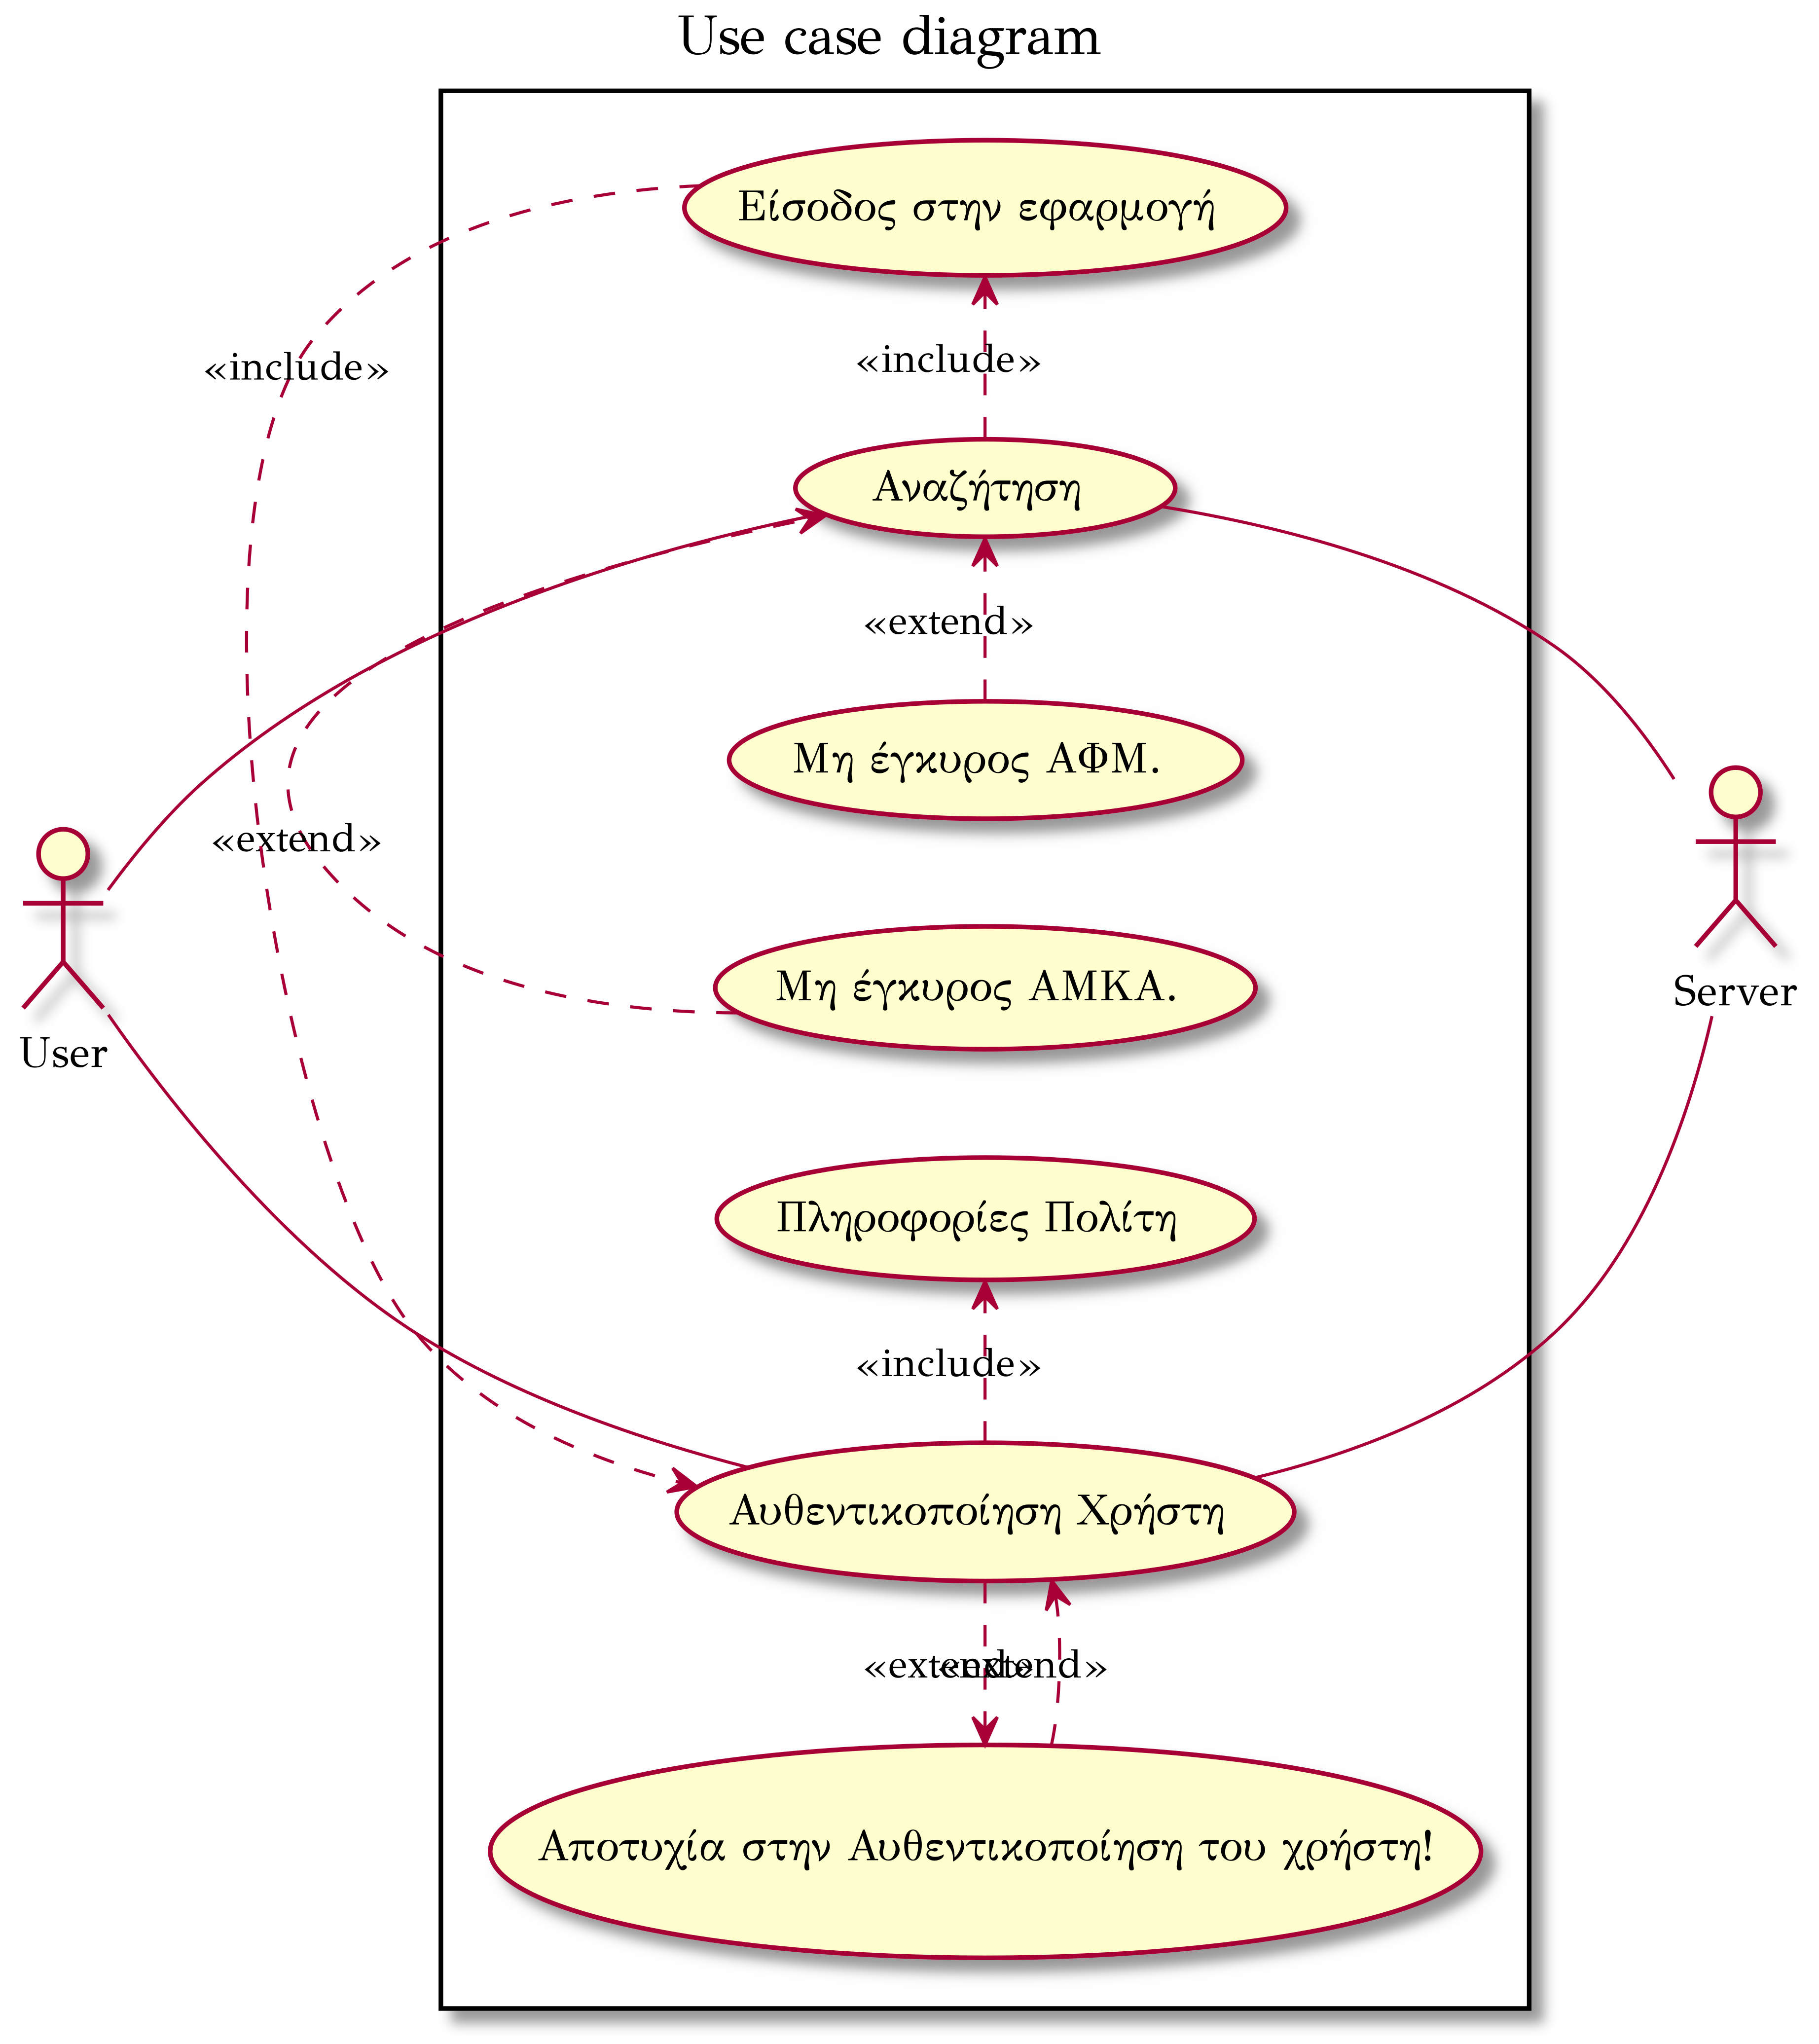
\includegraphics[scale=0.9]{use_case_diagram.png}
\end{center}


\section{Ερώτηση 4}
\textbf{Βασισμένοι στην απάντηση της ερώτησης 2 και 3 σχεδιάστε ένα πλήρες ΔΙΑΓΡΑΜΜΑ ΚΛΑΣΕΩΝ UML σε επίπεδο λεπτομέρειας σταδίου σχεδιασμού λογισμικού }

\begin{center}
    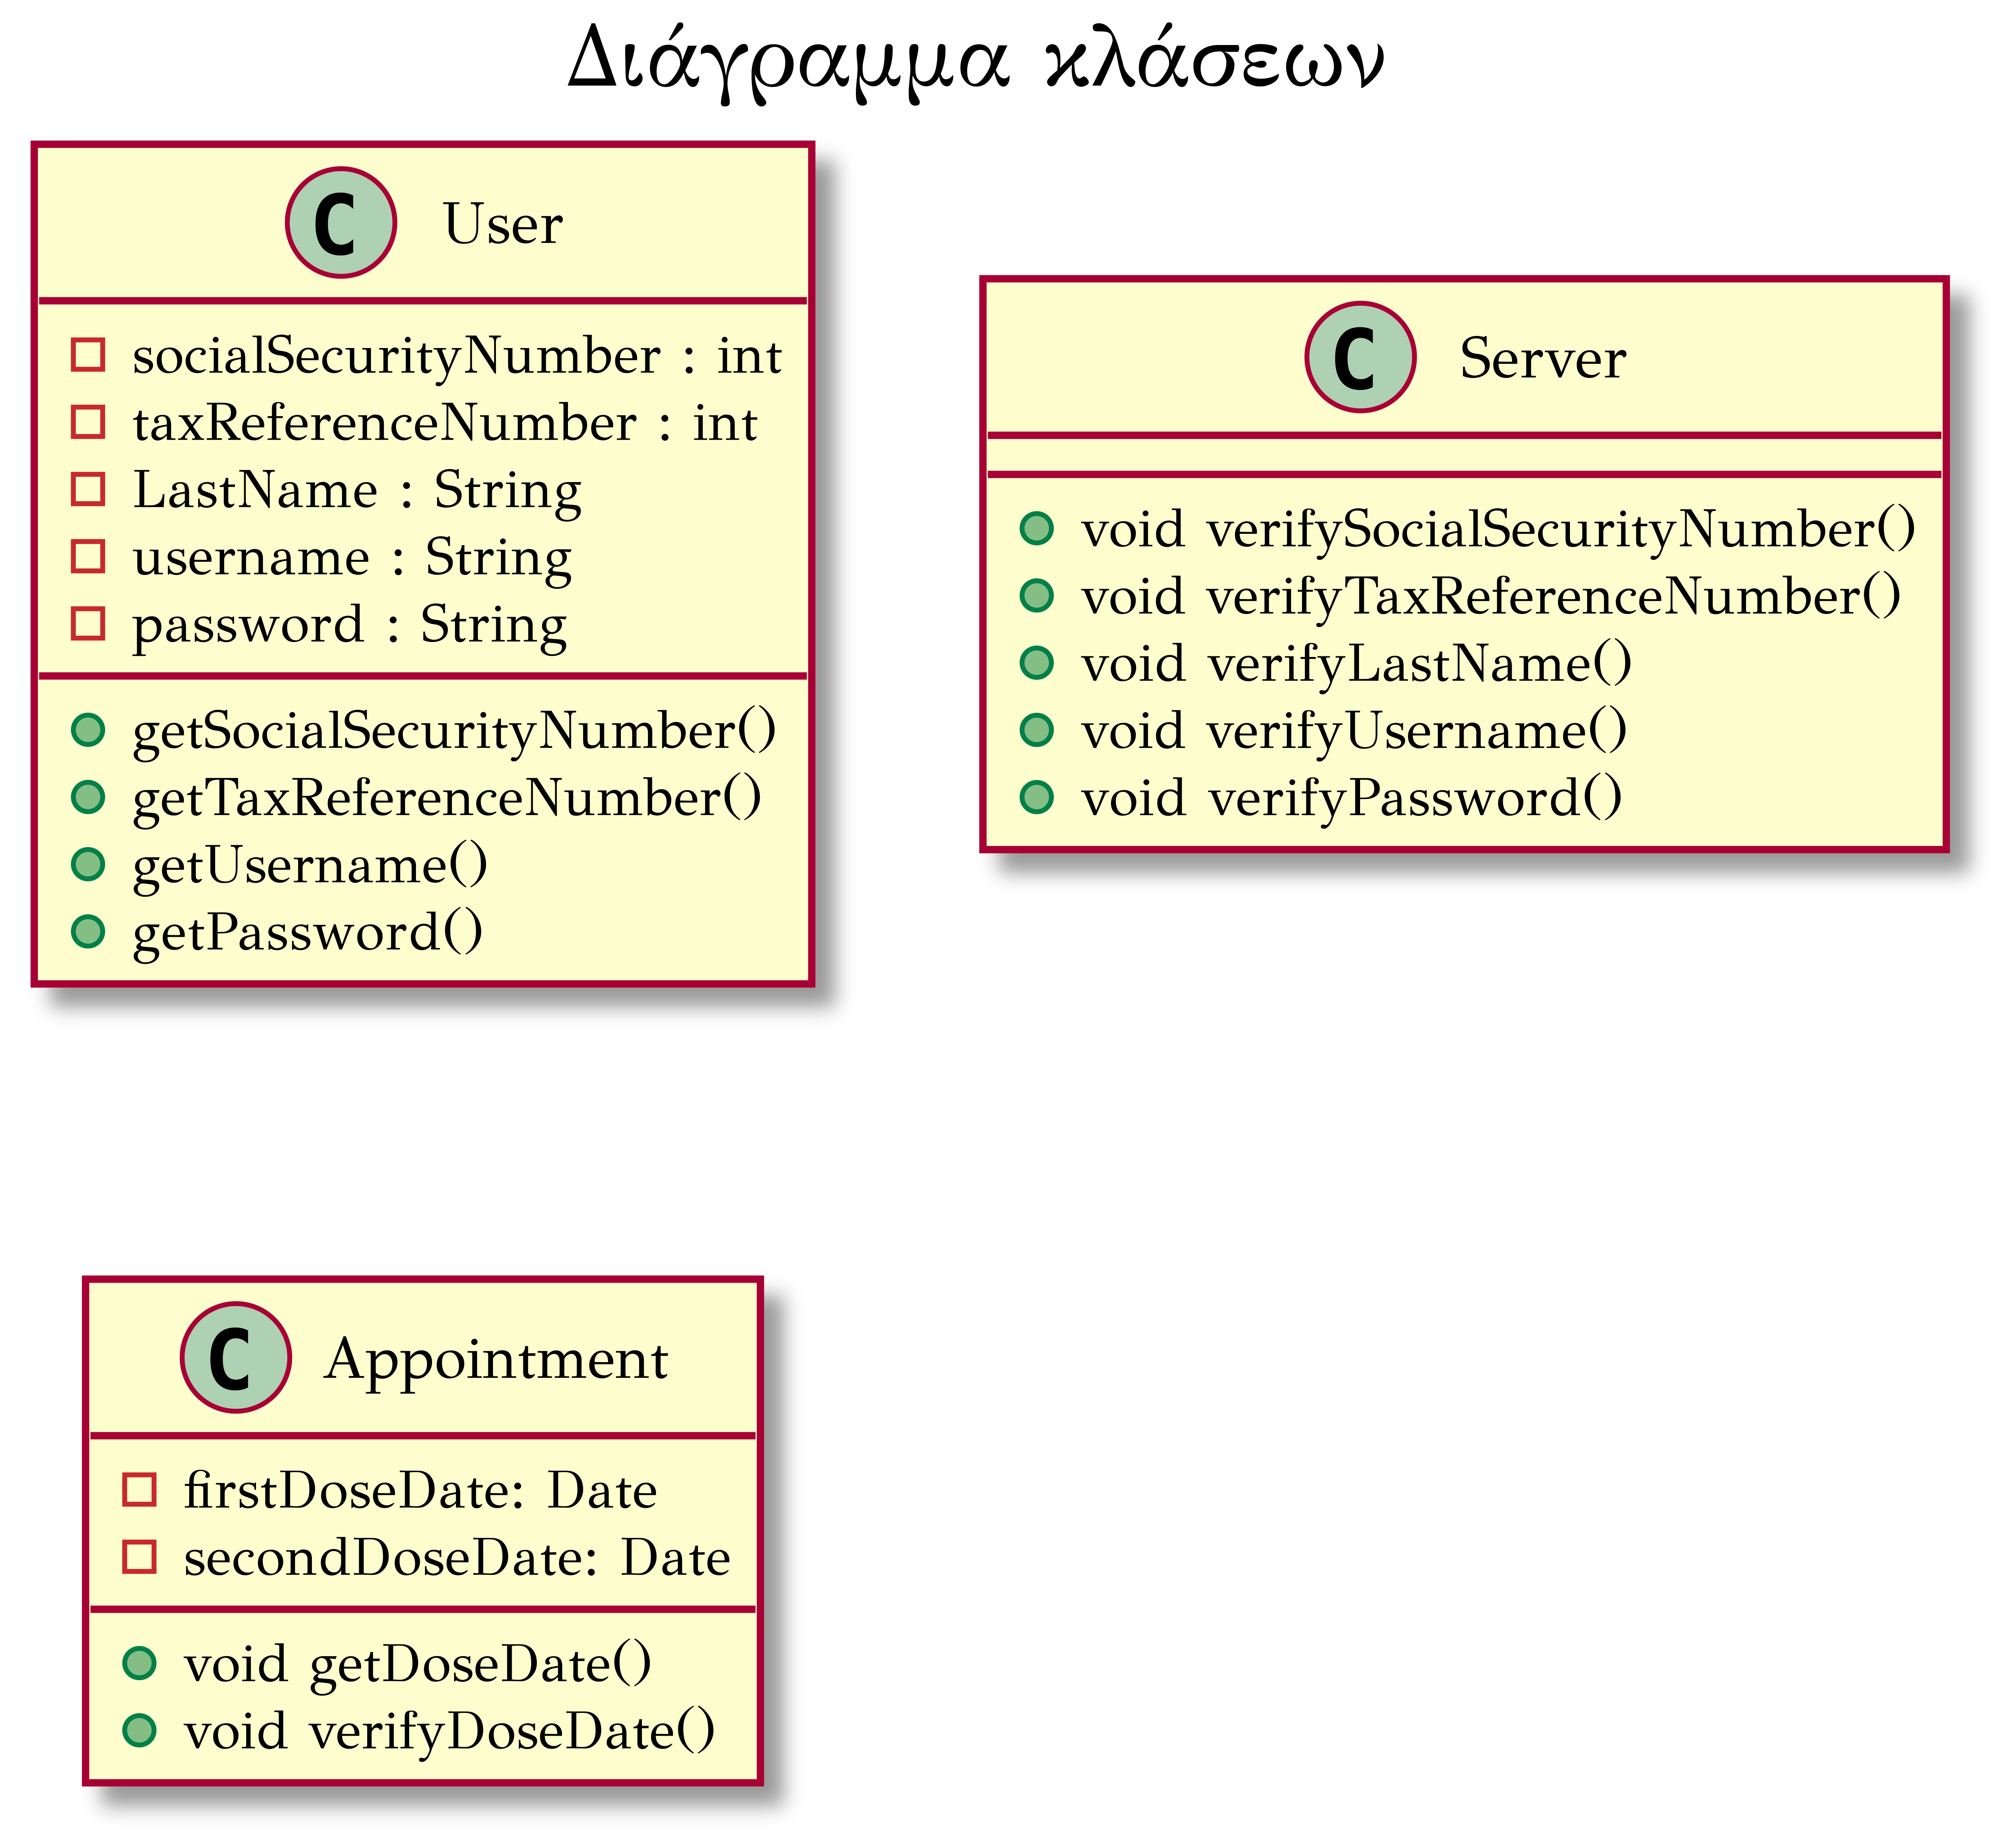
\includegraphics[scale=0.6]{class_diagram.png}
\end{center}

\newpage
\section{Πάσο}


\includegraphics[scale=0.09]{id_front.jpg}

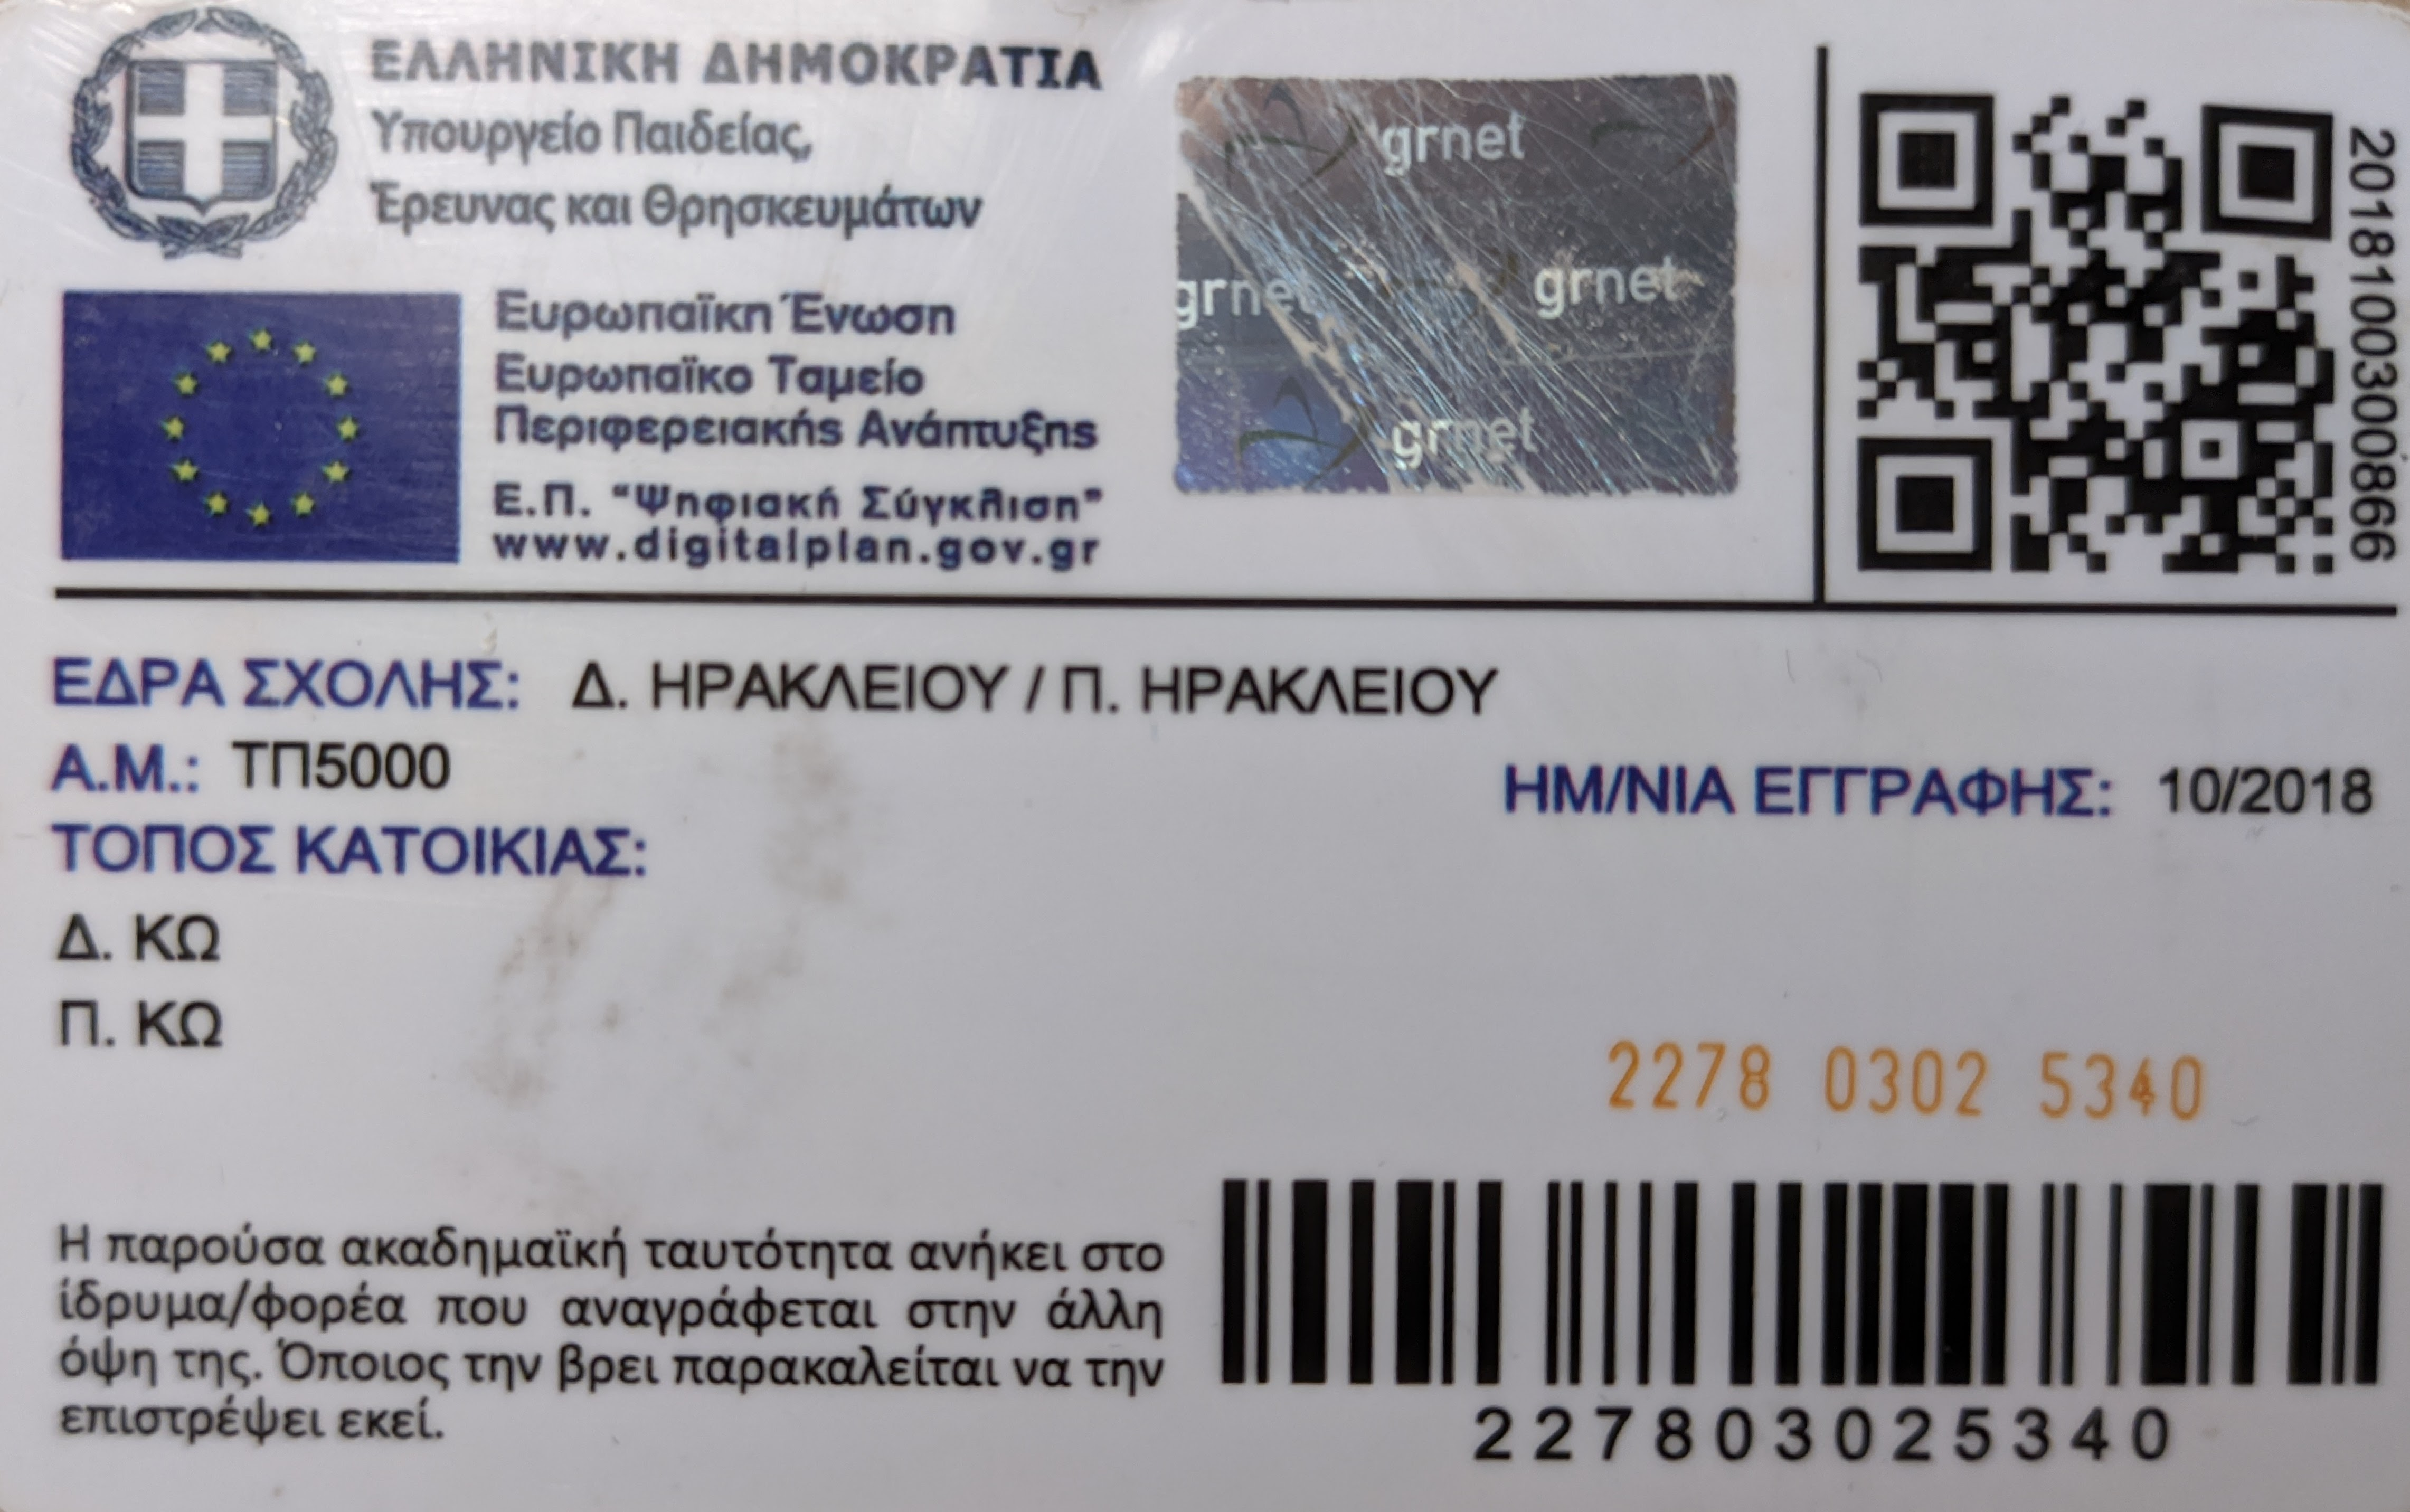
\includegraphics[scale=0.09]{id_back.jpg}

\end{document}